\documentclass[a4paper, 12pt]{report}

%%%%%%%%%%%%
% Packages %
%%%%%%%%%%%%

\usepackage{./Nyx/nyx-packages}
\usepackage{./Nyx/nyx-styles}
\usepackage{./Nyx/nyx-frames}
\usepackage{./Nyx/nyx-title}
\usepackage{./Nyx/nyx-macros}

%%%%%%%%%%%%%%
% Title-page %
%%%%%%%%%%%%%%

\logo{./Nyx/logo.png}

\institute{\curlyquotes{\hspace{0.25mm}Sapienza} Università di Roma}
\faculty{Ingegneria dell'Informazione,\\Informatica e Statistica}
\department{Dipartimento di Informatica}

\title{Automi: Calcolabilità e Complessità}
\subtitle{Appunti integrati con il libro "Introduzione alla teoria della computazione", Michael Sipser}

% \author{\textit{Author}\\TODO: DECOMMENTARE QUESTA SEZIONE}
% \author{\textit{Author}\\Simone Bianco}
\author{\textit{Author}\\Alessio Bandiera}
% \supervisor{Linus \textsc{Torvalds}}
% \context{Well, I was bored\ldots}

\date{\today}

%%%%%%%%%%%%
% Document %
%%%%%%%%%%%%

\begin{document}
    \maketitle

    % The following style changes are valid only inside this scope 
    {
        \hypersetup{allcolors=black}
        \fancypagestyle{plain}{%
        \fancyhead{}        % clear all header fields
        \fancyfoot{}        % clear all header fields
        \fancyfoot[C]{\thepage}
        \renewcommand{\headrulewidth}{0pt}
        \renewcommand{\footrulewidth}{0pt}}

        \romantableofcontents
    }

    \chapter*{Informazioni e Contatti}      % \chapter* makes this a "fake" chapter
    \markboth{Informazioni e Contatti}{}    % Manually sets \leftmark (current chapter name)
    \addcontentsline{toc}{chapter}{Informazioni e Contatti}     % Manually adds chapter to ToC
    
    \subsubsection{Prerequisiti consigliati:}
    \begin{itemize}
        \item TODO: DA DECIDERE
    \end{itemize}

    \quad

    \subsubsection{Segnalazione errori ed eventuali migliorie:}
    
    Per segnalare eventuali errori e/o migliorie possibili, si prega di utilizzare il \textbf{sistema di Issues fornito da GitHub} all'interno della pagina della repository stessa contenente questi ed altri appunti (link fornito al di sotto), utilizzando uno dei template già forniti compilando direttamente i campi richiesti.

    Gli appunti sono in continuo aggiornamento, pertanto, previa segnalazione, si prega di controllare se l'errore sia ancora presente nella versione più recente.

    \quad

    \subsubsection{Licenza di distribuzione:}
    
    These documents are distributed under the \textbf{\href{https://www.gnu.org/licenses/fdl-1.3.txt}{GNU Free Documentation License}}, a form of copyleft intended to be used on manuals, textbooks or other types of document in order to assure everyone the effective freedom to copy and redistribute it, with or without modifications, either commercially or non-commercially.
    
    \quad

    \subsubsection{Contatti dell'autore e ulteriori link:}
    \begin{itemize}
        % \item TODO: DECOMMENTARE QUESTA SEZIONE

        % Simone
        % 
        % \item Altri appunti: \textbf{\href{https://github.com/Exyss/university-notes}{https://github.com/Exyss/university-notes}}
        % \item Github: \textbf{\href{https://github.com/Exyss}{https://github.com/Exyss}}
        % \item Email: \textbf{\href{mailto:bianco.simone@outlook.it}{bianco.simone@outlook.it}}
        % \item LinkedIn: \textbf{\href{https://www.linkedin.com/in/simone-bianco}{Simone Bianco}}

        % Alessio
        % 
        \item Github: \textbf{\href{https://github.com/ph04}{https://github.com/ph04}}
        \item Email: \textbf{\href{mailto:alessio.bandiera02@gmail.com}{alessio.bandiera02@gmail.com}}
        \item LinkedIn: \textbf{\href{https://www.linkedin.com/in/alessio-bandiera-a53767223/}{Alessio Bandiera}}
    \end{itemize}

    %%%%%%%%%%%%%%%%%%%%%

    \chapter{Linguaggi regolari}

    \section{Automi finiti}

    \subsection{Linguaggi}

    \begin{frameddefn}{Alfabeto}
        Si definisce \textbf{alfabeto} un qualsiasi insieme finito, non vuoto; i suoi elementi sono detti \textbf{simboli}.
    \end{frameddefn}

    \begin{example}[Alfabeto]
        $\Sigma = \{\ttt 0,\ttt 1,\ttt x,\ttt y,\ttt z\}$ è un alfabeto, composto da 5 simboli.
    \end{example}

    \begin{frameddefn}{Stringa}
        Sia $\Sigma$ un alfabeto; una \textbf{stringa su $\Sigma$} è una sequenza finita di simboli di $\Sigma$; la \textbf{stringa vuota} appartiene ad ogni alfabeto, ed è denotata con $\varepsilon$.

        \begin{itemize}
            \item Data una stringa $w$ di $\Sigma$, allora $|w|$ è la lunghezza di $w$.
            \item Se $w$ ha lunghezza $n \in \mathbb{N}$, allora è possibile scrivere che $w = w_1 w_2 \cdots w_n$ con $w_i \in \Sigma$ e $i \in [1, n]$.
        \end{itemize}
    \end{frameddefn}

    \begin{example}[Stringa]
        Sia $\Sigma = \{\ttt 0,\ttt 1,\ttt x,\ttt y,\ttt z\}$ un alfabeto; allora una sua possibile stringa è $w = \ttt x \ttt 1 \ttt y \ttt 0 \ttt z$.
    \end{example}

    \begin{frameddefn}{Stringa inversa}
        Sia $\Sigma$ un alfabeto, e $w = w_1 w_2\cdots w_n$ una sua stringa; allora si definisce l'\textbf{inversa} di $w$ come segue: $w^\mathcal{R}= w_n w_{n - 1}\cdots w_1$
    \end{frameddefn}

    \begin{frameddefn}{Concatenazione}
        Sia $\Sigma$ un alfabeto, e $x = x_1 x_2 \cdots x_n, y = y_1 y_2 \cdots y_n$ due sue stringhe; allora $xy$ è la stringa ottenuta attraverso la \textbf{concatenazione} di $x$ ed $y$.

        Per indicare una stringa concatenata con se stessa $k$ volte, si utilizza la notazione $x^k = \underbrace{xx \cdots x}_k$.
    \end{frameddefn}

    \begin{frameddefn}{Prefisso}
        Sia $\Sigma$ un alfabeto, ed $x, y$ due sue stringhe; allora $x$ è detto essere un \textbf{prefisso} di $y$, se $\exists z \mid xz = y$, con $z$ stringa in $\Sigma$.
    \end{frameddefn}

    \begin{example}[Prefisso]
        Sia $\Sigma = \{\ttt a,\ttt  b,\ttt  c\}$ un alfabeto; allora la stringa $x = \ttt{ab}$ è prefisso della stringa $y = \ttt{abc}$, poiché esiste una stringa $z = \ttt c$ tale per cui $xz = y$.
    \end{example}
    
    \begin{frameddefn}{Linguaggio}
        Sia $\Sigma$ un alfabeto; si definisce \textbf{linguaggio} un insieme di stringhe di $\Sigma$. Un linguaggio è detto \textbf{prefisso}, se nessun suo elemento è prefisso di un altro.
    \end{frameddefn}

    \subsection{Automi finiti}

    \begin{frameddefn}{Automa finito}
        Un \textbf{automa finito}, o \textbf{macchina}, è una quintupla $(Q, \Sigma, \delta, q_0, F)$, dove

        \begin{itemize}
            \item $Q$ è l'\textbf{insieme degli stati} dell'automa, un insieme \textit{finito}
            \item $\Sigma$ è l'\textbf{alfabeto} dell'automa, un insieme \textit{finito}
            \item $\func{\delta}{Q \times \Sigma}{Q}$ è la \textbf{funzione di transizione}, che definisce la relazione tra gli stati
            \item $q_0 \in Q$ è lo \textbf{stato iniziale}
            \item $F \subseteq Q$ è l'\textbf{insieme degli stati accettanti}, sui quali le stringhe possono terminare
        \end{itemize}

    \end{frameddefn}

    \begin{example}[Automa finito]
        Un esempio di automa finito è il seguente:

        \begin{figure}[H]
            \centering
            \begin{tikzpicture}[->,>=stealth,shorten >=1pt,auto,node distance=3cm,thick,main node/.style={scale=0.9,circle,draw,font=\sffamily\normalsize}]
                \node[initial,state] (1) {$q_1$};
                \node[state,accepting] (2) [right of=1] {$q_2$};
                \node[state] (3) [right of=2] {$q_3$};
     
                \path[every node/.style={font=\sffamily\small}]
                    (1) edge [bend left] node {\ttt 1} (2)
                    (2) edge [bend left] node {\ttt 0} (3)
                    (3) edge [bend left] node {\ttt{0,1}} (2)
                    (1) edge [loop above] node {\ttt 0} (1)
                    (2) edge [loop above] node {\ttt 1} (2)
                 ;
             \end{tikzpicture}
             \caption{Un automa finito.}
        \end{figure}

        esso può essere descritto secondo la quintupla $(Q, \Sigma, \delta, q_0, F)$ come segue:

        \begin{itemize}
            \item $Q = \{q_1, q_2, q_3\}$
            \item $\Sigma = \{\ttt 0, \ttt 1\}$
            \item $\delta$ è la seguente: \begin{center} \begin{tabular}{c|cc} & \ttt 0 & \ttt 1 \\ \hline $q_1$ & $q_1$ & $q_2$ \\$q_2$ & $q_3$ & $q_2$ \\ $q_3$ & $q_2$ & $q_2$ \end{tabular} \end{center}
            \item $q_1$ è lo stato iniziale
            \item $F = \{q_2\} \subseteq Q$
        \end{itemize}
    \end{example}

    \begin{frameddefn}{Linguaggio di un automa}
        Sia $M$ un automa; allora il \textbf{linguaggio} di $M$ è un insieme $L(M)$ contenente tutte le stringhe accettate da $M$; simmetricamente, si dice che $M$ \textbf{riconosce} $L(M)$.
    \end{frameddefn}

    \begin{example}[Linguaggio di un automa]
        Si consideri il seguente automa $M_1$:

        \begin{figure}[H]
            \centering
            \begin{tikzpicture}[->,>=stealth,shorten >=1pt,auto,node distance=3cm,thick,main node/.style={scale=0.9,circle,draw,font=\sffamily\normalsize}]
                \node[initial,state] (1) {$q_1$};
                \node[state,accepting] (2) [right of=1] {$q_2$};

                \path[every node/.style={font=\sffamily\small}]
                    (1) edge [bend left] node {\ttt 1} (2)
                    (2) edge [bend left] node {\ttt 0} (1)
                    (1) edge [loop above] node {\ttt 0} (1)
                    (2) edge [loop above] node {\ttt 1} (2)
                 ;
             \end{tikzpicture}
             \caption{Un automa $M_1$.}
        \end{figure}

        sapendo che $\Sigma = \{\ttt 0, \ttt 1\}$, che $q_1$ è lo stato iniziale, e che $F = \{q_2\}$, ci si convince facilmente che $$L(M_1) = \{w \mid w = w_1 w_2 \cdots w_{n - 1} \ttt{1}, n \in \mathbb{N}\}$$ ovvero, $M_1$ accetta tutte e sole le stringhe che terminano per \ttt 1.
    \end{example}

    \begin{frameddefn}{Stringhe accettate}
        Sia $M = (Q, \Sigma, \delta, q_0, F)$ un automa, e sia $w = w_1\cdots w_n$ una stringa tale per cui $\forall i \in [1, n] \quad w_i \in \Sigma$; allora, $M$ \tbf{accetta} $w$ se esiste una sequenza di stati $r_0, \ldots, r_n \in Q$ tali per cui

        \begin{itemize}
            \item $r_0 = q_0$
            \item $\forall i \in [1, n - 1] \quad \delta(r_i, w_{i + 1})=r_{i + 1}$
            \item $r_n \in F$
        \end{itemize}

        Dato un linguaggio $A$, si ha che $M$ \tbf{riconosce} $A$ se e solo se $A = \{w \mid M \ \mathrm{accetta} \ w\}$.
    \end{frameddefn}

    \begin{frameddefn}{Linguaggio regolare}
        Un linguaggio è detto \tbf{regolare} se e solo se esiste un automa finito che lo riconosce.
    \end{frameddefn}

    \section{Non determinismo}

    \subsection{Definizioni}
    
    \begin{frameddefn}{NFA}
        Un \tbf{NFA} (\tit{Nondeterministic Finite Automaton}) è un automa in cui possono esistere varie scelte per lo stato successivo in ogni punto. Durante la computazione, ogni volta che viene incontrata una scelta, la macchina si \tit{divide}, e ognuno dei vari automi risultanti computa le varie scelte indipendentemente.

        Formalmente, un NFA è una quintupla $(Q, \Sigma, \delta, q_0, F)$, dove

        \begin{itemize}
            \item $Q$ è l'\tbf{insieme degli stati}, un insieme \tit{finito}
            \item $\Sigma$ è l'\tbf{alfabeto} dell'automa, un insieme \tit{finito}
            \item $\delta: Q \times \Sigma_{\varepsilon} \rightarrow \mathcal{P}(Q)$ è la \tbf{funzione di transizione}, che definisce la relazione tra gli stati
            \item $q_0 \in Q$ è lo \tbf{stato iniziale}
            \item $F \subseteq Q$ è l'\tbf{insieme degli stati accettanti}
        \end{itemize}

        dove $\Sigma_{\varepsilon} := \Sigma \cup \{\varepsilon\}$.

        Se il simbolo di input successivo non compare su alcuno degli archi uscenti dallo stato occupato da una copia della macchina, quella copia cessa di proseguire; inoltre, se \tit{una qualunque copia} della macchina è in uno stato accettante, l'NFA accetta la stringa di input. Si noti che questa divisione è descritta dall'insieme potenza $\mathcal{P}(Q)$, poiché da ogni stato si può arrivare ad un \tit{insieme} di stati.

        Gli automi deterministici vengono anche detti \tbf{DFA} (\tit{Deterministic Finite Automaton}). Si noti che il determinismo è un caso particolare di non determinismo, dunque un DFA è sempre anche un NFA.
    \end{frameddefn}

    \begin{example}[NFA]
        Un esempio di NFA è il seguente:

        \begin{figure}[H]
            \centering
            \begin{tikzpicture}[->,>=stealth,shorten >=1pt,auto,node distance=3cm,thick,main node/.style={scale=0.9,circle,draw,font=\sffamily\normalsize}]
                \node[initial,state] (1) {$q_1$};
                \node[state] (2) [right of=1] {$q_2$};
                \node[state] (3) [right of=2] {$q_3$};
                \node[state,accepting] (4) [right of=3] {$q_4$};

                \path[every node/.style={font=\sffamily\small}]
                    (1) edge [loop above] node {\ttt{0,1}} (1)
                    (1) edge node {\ttt 1} (2)
                    (2) edge node {\ttt{0,} $\varepsilon$} (3)
                    (3) edge node {\ttt 1} (4)
                    (4) edge [loop above] node {\ttt{0,1}} (4)
                 ;
             \end{tikzpicture}
             \caption{Un NFA.}

        \end{figure}

        esso può essere descritto secondo la quintupla $(Q, \Sigma, \delta, q_0, F)$ come segue:

        \begin{itemize}
            \item $Q = \{q_1, q_2, q_3, q_4\}$
            \item $\Sigma = \{\ttt 0, \ttt 1\}$
            \item $\delta$ è la seguente: \begin{center} \begin{tabular}{c|ccc} & \ttt 0 & \ttt 1 & $\varepsilon$ \\ \hline $q_1$ & $\{q_1\}$ & $\{q_1, q_2\}$ & $\varnothing$ \\ $q_2$ & $\{q_3\}$ & $\varnothing$ & $\{q_3\}$ \\ $q_3$ & $\varnothing$ & $\{q_4\}$ & $\varnothing$ \\ $q_4$ & $\{q_4\}$ & $\{q_4\}$ & $\varnothing$ \end{tabular} \end{center}
            \item $q_1$ è lo stato iniziale
            \item $F = \{q_4\} \subseteq Q$
        \end{itemize}

        L'esecuzione dell'NFA mostrato è la seguente:

        \begin{center}
            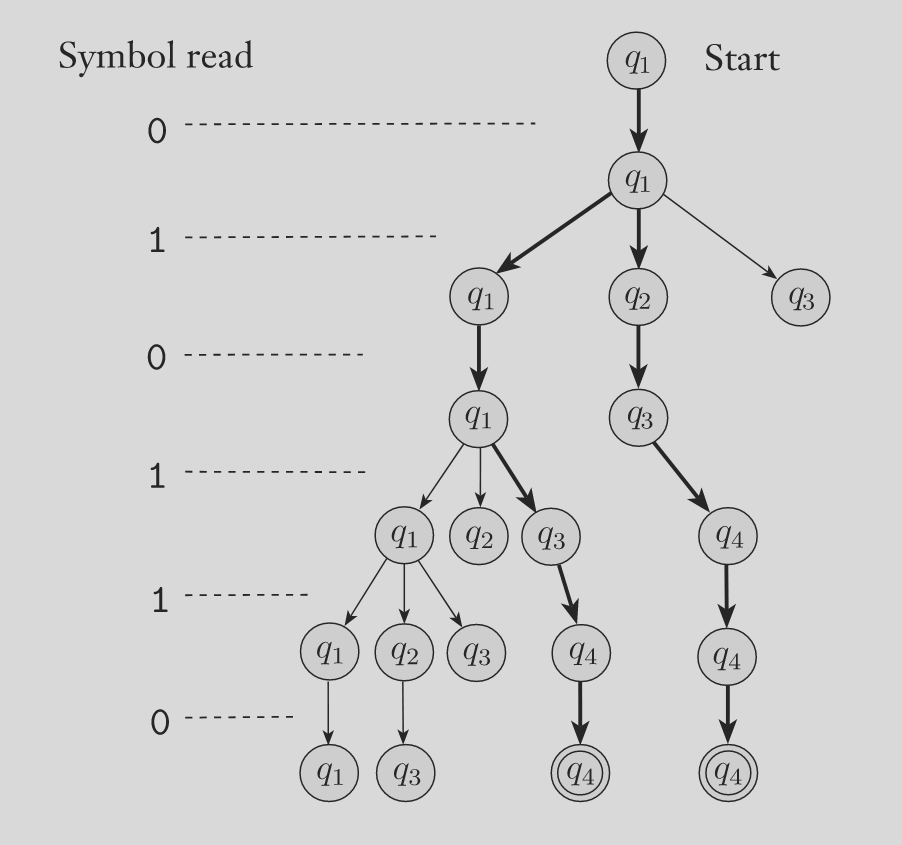
\includegraphics[scale=0.4]{assets/nfa-neg.png}
        \end{center}

        Si noti che nel momento in cui vengono incontrati $\varepsilon$-archi si giunge allo stato successivo nello stesso step dell'input incontrato, dunque gli $\varepsilon$-archi \tit{non} producono uno step di esecuzione, ma vengono eseguiti non appena vengono incontrati, e vengono accorpati immediatamente.
    \end{example}

    \begin{frameddefn}{Stringhe accettate}
        Sia $N = (Q, \Sigma, \delta, q_0, F)$ un automa, e sia $w = w_1\cdots w_n$ una stringa tale per cui $\forall i \in [1, n] \quad w_i \in \Sigma$; allora, $M$ \tbf{accetta} $w$ se esiste una sequenza di stati $r_0, \ldots, r_n \in Q$ tali per cui

        \begin{itemize}
            \item $r_0 = q_0$
            \item $\forall i \in [1, n - 1] \quad r_{i + 1} \in \delta(r_i, w_{i + 1})$
            \item $r_n \in F$
        \end{itemize}
    \end{frameddefn}

    \begin{frameddefn}{Equivalenza tra automi}
        Due macchine si dicono \tbf{equivalenti} se e solo se riconoscono lo stesso linguaggio.
    \end{frameddefn}

    \begin{framedthm}[label={nfa equiv}]{DFA equivalente ad NFA}
        Sia $N$ un NFA; allora, esiste un DFA ad esso equivalente.
    \end{framedthm}

    \begin{proof}
        Sia $N = (Q, \Sigma_{\varepsilon}, \delta, q_0, F)$ l'NFA in ipotesi, tale da riconoscere un linguaggio A. Inoltre, si definisca $$\forall k \ge 0 \quad \displaystyle E(R) := \bigcup_{r \in R}{\delta^k(r, \varepsilon)}$$ l'insieme degli stati raggiungibili da stati in $R$, applicando (anche ripetutamente) un numero arbitrario di $\varepsilon$-archi (si noti che per $k = 0$ si ha che $R \subseteq E(R)$).

        Allora, sia $M = (Q', \Sigma_{\varepsilon}, \delta', q_0', F)$ il DFA definito come segue:

        \begin{itemize}
            \item $Q' := \powerset{(Q)}$, scelto tale da rappresentare ogni possibile stato di $N$;
            \item $\displaystyle \forall R \in Q', a \in \Sigma \quad \delta'(R, a) := \bigcup_{r \in R}{E(\delta(r, a))}$, scelta tale in quanto, per un certo insieme di stati $R \in Q'$ di $N$, a $\delta'(R, a)$ viene assegnata l'unione degli stati che sarebbero stati raggiunti in $N$ dagli $r \in R$ con $a$, calcolati dunque attraverso $\delta(r, a)$, aggiungendo infine i possibili $\varepsilon$-archi;
            \item $q_0' := E(\{q_0\})$, scelto tale da far iniziare $M$ esattamente dove aveva inizio $N$, comprendendo anche i possibili $\varepsilon$-archi iniziali;
            \item $F' := \{R \in Q' \mid \exists r \in R : r \in F\}$, che corrisponde all'insieme degli insiemi di stati di $N$ contenenti almeno uno stato accettante in $N$.
        \end{itemize}

        Allora $M$ è in grado di riconoscere $A$ per costruzione, poiché il DFA costruito emula l'NFA di partenza, tenendo anche in considerazione gli $\varepsilon$-archi. Dunque, sia $N$ che $M$ riconoscono $A$, e per definizione sono di conseguenza equivalenti.
    \end{proof}
    
    \begin{framedcor}{Linguaggi regolari con NFA}
        Sia $A$ un linguaggio; allora, $A$ è regolare se e solo se esiste un NFA che lo riconosce.
    \end{framedcor}

    \proofiff{
        Per definizione, $A$ è regolare, dunque esiste un DFA che lo riconosce. Allora, poiché un DFA è sempre anche NFA, segue la tesi.
    }{
        Sia $A$ un linguaggio tale da essere riconosciuto da un NFA; allora, per il TODO FIXA STA ROBA NON FUNZIONA \Cref{nfa equiv}, esiste un DFA equivalente all'NFA che riconosce $A$, e dunque per definizione $A$ è regolare.
    }

    \section{Operazioni regolari}

    \subsection{Definizioni}
    
    \begin{frameddefn}{Unione}
        Siano $A$ e $B$ due linguaggi; allora, si definisce l'\tbf{unione} di $A$ e $B$ il seguente linguaggio: $$A \cup B = \{x \mid x \in A \lor x \in B \}$$
    \end{frameddefn}

    \begin{example}[Unione]
        Sia $\Sigma = \{\ttt a , \ldots, \ttt z\}$ l'alfabeto composto da 26 lettere, e siano $A = \{\ttt{uno}, \ttt{due}\}$ e $B = \{\ttt{tre}, \ttt{quattro}\}$ due linguaggi su $\Sigma$. Allora, si ha che $$A \cup B = \{\ttt{uno}, \ttt{due}, \ttt{tre}, \ttt{quattro}\}$$
    \end{example}

    \begin{framedprop}{Chiusura dell'unione}
        Siano $A$ e $B$ due linguaggi regolari su un alfabeto $\Sigma$; allora $A \cup B$ è regolare.
    \end{framedprop}

    \begin{proof}[Dimostrazione I]
        Per definizione, $A$ e $B$ sono linguaggi regolari, dunque esistono due automi finiti $$\left. \begin{array}{c}M_1 = (Q_1, \Sigma, \delta_1, q_1, F_1) \\ M_2 = (Q_2, \Sigma, \delta_2, q_2, F_2)\end{array} \right.$$ tali da riconoscere rispettivamente $A$ e $B$. Allora, sia $M = (Q, \Sigma, \delta, q_0, F)$ l'automa finito definito come segue:

        \begin{itemize}
            \item $Q := Q_1 \times Q_2 = \{(r_1, r_2) \mid r_1 \in Q_1 \land r_2 \in Q_2\}$, scelto tale in quanto permette di avere tutte le possibili combinazioni di stati dei due automi di partenza;
            \item $\forall (r_1, r_2) \in Q, a \in \Sigma \quad \delta((r_1, r_2), a) := (\delta_1(r_1, a), \delta_2(r_2, a))$, scelta tale in quanto permette di simulare entrambi gli automi di partenza contemporaneamente, mandando ogni stato di $M_1$ ed $M_2$ dove sarebbe andato nei rispettivi automi di appartenenza;
            \item $q_0 := (q_1, q_2)$, scelto tale in quanto deve essere lo stato in cui entrambe gli automi in ipotesi iniziavano;
            \item $F := (F_1 \times Q_2) \cup (Q_1 \times F_2) = \{(r_1, r_2) \mid r_1 \in F_1 \lor r_2 \in F_2\}$, scelto tale in quanto permette di simulare gli stati accettanti di entrambi gli automi, e vanno prese tutte le coppie che vedono almeno uno dei due stati come accettanti poiché altrimenti non si accetterebbero delle stringhe accettate da $M_1$ ed $M_2$ in partenza.
        \end{itemize}

        Allora, poiché $M$ è in grado di simulare $M_1$ ed $M_2$ contemporaneamente, per costruzione accetterà ogni stringa di $A$ e di $B$, dunque riconoscendo $A \cup B$, e di conseguenza $A \cup B$ è regolare per definizione.
    \end{proof}

    \begin{proof}[Dimostrazione II]
        Siano $N_1$ ed $N_2$ i seguenti NFA, tali da riconoscere rispettivamente i due linguaggi $A$ e $B$ in ipotesi: $$\left . \begin{array}{c}N_1 = (Q_1, \Sigma, \delta_1, q_1, F_1) \\ N_2 = (Q_2, \Sigma, \delta_2, q_2, F_2) \end{array} \right .$$ Allora, sia $N = (Q, \Sigma, \delta, q_0, F)$ l'NFA costruito come segue:

        \begin{itemize}
            \item $Q = \{q_0\} \cup Q_1 \cup Q_2$, dove $q_0$ è un nuovo stato, e $Q$ è scelto tale da includere sia $N_1$ che $N_2$;
            \item $\forall q \in Q, a \in \Sigma_{\varepsilon} \quad \delta(q, a) = \left \{ \begin{array}{ll} \delta_1(q, a) & q \in Q_1 \\ \delta_2(q, a) & q \in Q_2 \\ \{q_1, q_2\} & q = q_0 \land a = \varepsilon \\ \varnothing & q = 0 \land a \neq \varepsilon \end{array} \right.$, scelta tale da poter eseguire contemporaneamente gli NFA $N_1$ ed $N_2$, definendo per casi la funzione di transizione;
            \item $q_0$ è il nuovo stato, che rappresenta lo stato iniziale di $N$;
            \item $F = F_1 \cup F_2$, scelto tale da costruire $N$ in modo che accetti una stringa se e solo se la accetterebbero $N_1$ o $N_2$.
        \end{itemize}

        Allora, l'NFA risultante $N$ è in grado di computare contemporaneamente $N_1$ ed $N_2$, ed è dunque in grado di riconoscere $A$ e $B$ contemporaneamente; di conseguenza, $N$ riconosce $A \cup B$, che risulta dunque essere regolare per definizione.

        La foto seguente raffigura la dimostrazione costruttiva appena descritta:

        \begin{center}
            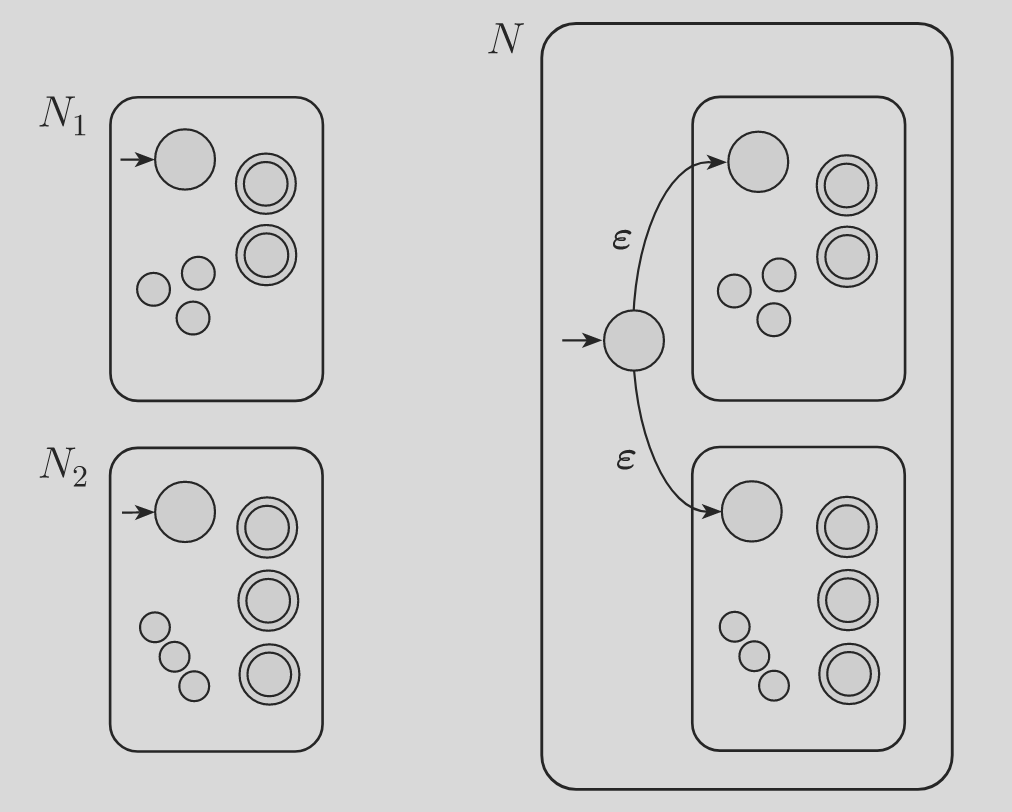
\includegraphics[scale=0.4]{assets/union-neg.png}
        \end{center}

    \end{proof}

    \begin{frameddefn}{Concatenazione}
        Siano $A$ e $B$ due linguaggi; allora, si definisce la \tbf{concatenazione} di $A$ e $B$ il seguente linguaggio: $$A \circ B = \{xy \mid x \in A \land y \in B\}$$
    \end{frameddefn}

    \begin{example}[Concatenazione]
        Sia $\Sigma = \{\ttt a , \ldots, \ttt z\}$ l'alfabeto composto da 26 lettere, e siano $A = \{\ttt{uno}, \ttt{due}\}$ e $B = \{\ttt{tre}, \ttt{quattro}\}$ due linguaggi su $\Sigma$. Allora, si ha che $$A \circ B = \{\ttt{unotre}, \ttt{unoquattro}, \ttt{duetre}, \ttt{duequattro}\}$$
    \end{example}

    \begin{framedprop}{Chiusura della concatenazione}
        Siano $A$ e $B$ due linguaggi regolari su un alfabeto $\Sigma$; allora $A \circ B$ è regolare.
    \end{framedprop}

    \begin{proof}
        TODO
    \end{proof}

    \begin{frameddefn}{Star}
        Sia $A$ un linguaggio; allora, si definisce l'operazione unaria \tbf{star} che definisce il seguente linguaggio: $$A^* = \{x_1 x_2 \cdots x_k \mid k \ge 0 \land \forall i \in [1, k] \quad x_i \in A\}$$

        Si noti che $k = 0 \implies \varepsilon \in A^*$ per ogni linguaggio $A$.
    \end{frameddefn}

    \begin{example}[Star]
        Sia $\Sigma = \{\ttt a , \ldots, \ttt z\}$ l'alfabeto composto da 26 lettere, e siano $A = \{\ttt{uno}, \ttt{due}\}$ e $B = \{\ttt{tre}, \ttt{quattro}\}$ due linguaggi su $\Sigma$. Allora, si ha che $$A^* = \{\varepsilon, \ttt{uno}, \ttt{due}, \ttt{unouno}, \ttt{unodue}, \ttt{dueuno}, \ttt{duedue}, \ldots\}$$
    \end{example}
   
    \begin{framedprop}{Chiusura dell'operazione star}
        Siano $A$ e $B$ due linguaggi regolari su un alfabeto $\Sigma$; allora $A^*$ è regolare.
    \end{framedprop}

    \begin{proof}
        Per definizione, $A$ e $B$ sono linguaggi regolari, dunque per l'\cref{nfa equiv} esistono due NFA $$\left. \begin{array}{c}N_1 = (Q_1, \Sigma, \delta_1, q_1, F_1) \\ N_2 = (Q_2, \Sigma, \delta_2, q_2, F_2) \end{array} \right.$$ tali da riconoscere rispettivamente $A$ e $B$. Allora, sia $N = (Q, \Sigma, \delta, q_0, F)$ l'NFA costruito come segue:

        \begin{itemize}
            \item TODO
        \end{itemize}
    \end{proof}
\end{document}
